\documentclass{article}

\usepackage[pdftex]{graphicx}
\usepackage{siunitx}

% *** CITATION PACKAGES ***
%
\usepackage{cite}
% cite.sty was written by Donald Arseneau
% V1.6 and later of IEEEtran pre-defines the format of the cite.sty package
% \cite{} output to follow that of the IEEE. Loading the cite package will
% result in citation numbers being automatically sorted and properly
% "compressed/ranged". e.g., [1], [9], [2], [7], [5], [6] without using
% cite.sty will become [1], [2], [5]--[7], [9] using cite.sty. cite.sty's
% \cite will automatically add leading space, if needed. Use cite.sty's
% noadjust option (cite.sty V3.8 and later) if you want to turn this off
% such as if a citation ever needs to be enclosed in parenthesis.
% cite.sty is already installed on most LaTeX systems. Be sure and use
% version 5.0 (2009-03-20) and later if using hyperref.sty.
% The latest version can be obtained at:
% http://www.ctan.org/pkg/cite
% The documentation is contained in the cite.sty file itself.



% *** MATH PACKAGES ***
%
\usepackage{amsmath}
% A popular package from the American Mathematical Society that provides
% many useful and powerful commands for dealing with mathematics.
%
% Note that the amsmath package sets \interdisplaylinepenalty to 10000
% thus preventing page breaks from occurring within multiline equations. Use:
\interdisplaylinepenalty=2500
% after loading amsmath to restore such page breaks as IEEEtran.cls normally
% does. amsmath.sty is already installed on most LaTeX systems. The latest
% version and documentation can be obtained at:
% http://www.ctan.org/pkg/amsmath



% correct bad hyphenation here
\hyphenation{op-tical net-works semi-conduc-tor}

%\usepackage[utf8]{inputenc}
%\usepackage{helvet}
%\usepackage[usenames,dvipsnames,svgnames,table]{xcolor}
%\usepackage{graphicx}
%\usepackage{caption}
%\usepackage{subcaption}
%\usepackage{url}
%\usepackage{amstext}

%\bibliographystyle{IEEEtran}

% Title Page
\title{Mapping Deforestation with Recurrence Metrics of Sentinel-1 time series}
\author{Felix Cremer, Mikhail Urbazaev, Christiane Schmullius and Christian Thiel}

%\IEEEauthorblockA{Chair of Earth Observation, Friedrich-Schiller University, Jena,Germany\\
%Email: felix.cremer@uni-jena.de}

\begin{document}
\maketitle
%\tableofcontents
\begin{abstract}
  Forest ecosystems
  REDD+ process
  order of time series
  SAR

%Keywords:Recurrence, SAR, time series, remote sensing
%
\end{abstract}
\section{Introduction}
The tropical forest ecosystems stabilise the world climate\cite{}, the protection of the biodiversity \cite{} and
for the well being of a vast amount of the global popu-
lation\cite{}.
 In the last decade remote sensing technologies have
played a substantial role in the consistent, reliable and timely
information gathering about forest cover changes. With the
REDD+ mechanism the use of remote sensing to monitor
and map deforestation and degradation processes has been
increased.
deforestation mapping based on Sentinel-1 data



\section{Method}

Recurrence plots have been proposed by Eckmann et al 1987. They are method to visualize the recurrences of a time series. They are a quadratic matrix which entries are defined as follows:
$$R_{i,j} = \Theta(\epsilon - \lvert x_i - x_j \rvert), i,j = 1,...,N$$
Figure \ref{rplots} shows an example Recurrence plot of stable forest and a deforested area.

\begin{\begin{figure}
  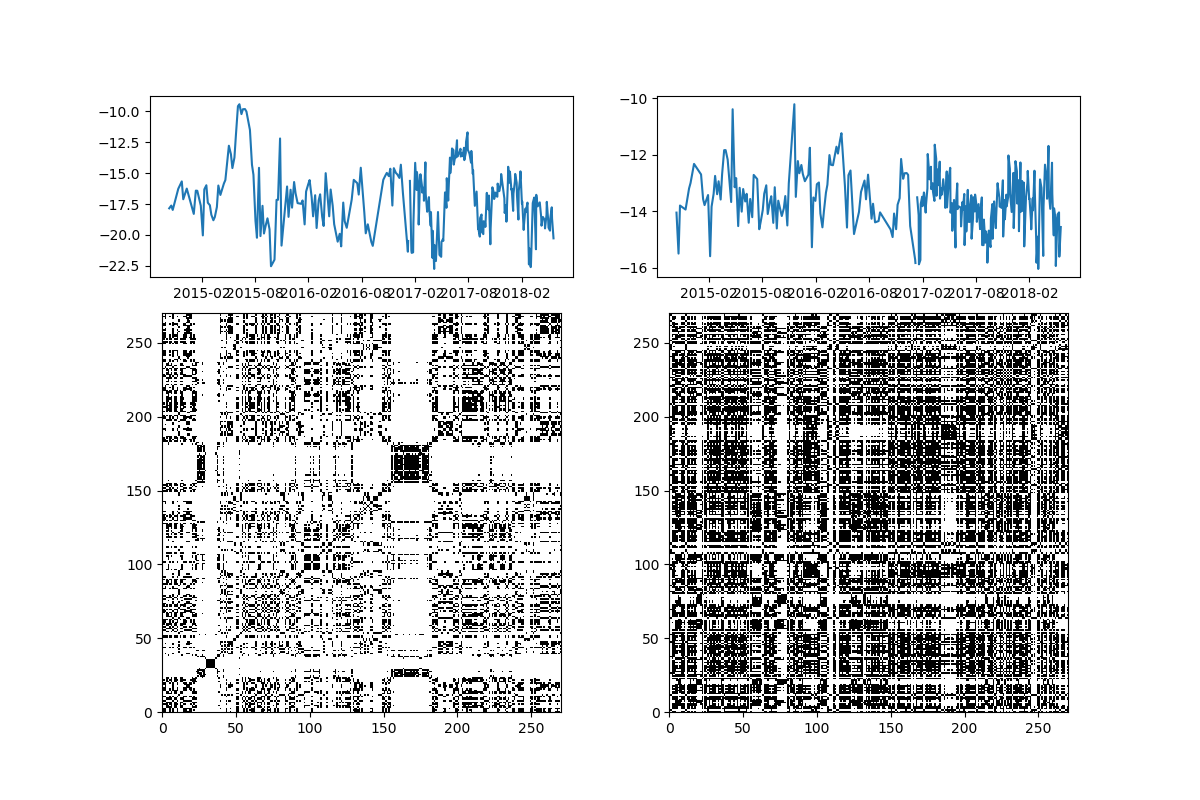
\includegraphics{figs/rpplot.png}
  \caption{Recurrence Plots for single pixel with stable forest and a deforested area.}
  \label{rplots}
\end{figure}}

\section{Experimental Results}
\subsection{Data and Preprocessing}
We test the separability of stable forest and deforestation on two testsites in Mexico.
One is mostly covered by temperate forests in central Mexico,
the other is situated on the Yucatan peninsula and is covered by tropical dry forests.

\color{red}{
The data have been preprocessed using the SNAP software \cite{SNAP}.
The single time steps are multilooked to a \SI{10}{\m} x \SI{10}{\m} pixel spacing.
The orthorectification is based on the original orbit state vectors and the \SI{30}{\m} SRTM digital elevation model\cite{SRTM}.
The preprocessing also included radiometric terrain flattening after \cite{Small} which results in $\gamma^0$ backscatter values.
All images were coregistered in the DEM geometry after geocoding to achieve a subpixel coregistration precision which is of eminent importance when the pixels are investigated in the temporal domain only.
}



\subsection{Separability analysis}

Show that the TREND metric is enhancing the separability of deforested areas and stable forests.
Quantify it.

\section{Discussion}

Do I need to do a comparison against optical deforestation maps?

\section{Summary and Conclusion}



\section*{Acknowledgment}
This work was funded by the DLR in the Sentinel4REDD project (FKZ:50EE1540).
This work uses Copernicus Sentinel data 2014-2018.



\bibliography{literatur}

\end{document}
